\documentclass{cmuthesis}
\usepackage{fullpage}
\usepackage[
  backref,pageanchor=true,plainpages=false, pdfpagelabels, bookmarks,bookmarksnumbered
]{hyperref}
\hypersetup{linktoc=all}
\usepackage{todonotes}
\usepackage{syntax}
\usepackage{amsmath}
\usepackage{wasysym}
\usepackage{subfigure}
\usepackage[numbers,sort]{natbib}
%\usepackage[letterpaper,twoside,vscale=.8,hscale=.75,nomarginpar,hmarginratio=1:1]{geometry}

\draftstamp{\today}{DRAFT}

\newcommand{\fyes}{\CIRCLE}
\newcommand{\fhalf}{\LEFTcircle}
\newcommand{\fno}{\Circle}

%I'll need to double space it for submission, but double
%spacing is a terrible relic of a time gone by, and hurts
%my eyes, so we'll turn it on later.
%\usepackage{setspace}
%\doublespacing
\begin{document}
\frontmatter
\pagestyle{empty}
% What a proposal should be, according to the ECE website
%    An explanation of the basic idea of the dissertation topic;
%    An explanation as to why this topic is interesting;
%    A statement as to what kind of results are expected, and;
%    A convincing argument as to why these results are attainable in a reasonable amount of time.
\newcommand{\sysname}{Holmes}
\title{\bf Thesis Proposal: \sysname}
\author{Matthew Maurer}
\Year{2015}
\trnumber{}

\committee{
David Brumley, Chair \\
Frank Pfenning \\
Lujo Bauer \\
Manuel Egele, Boston University 
}

\support{}
\disclaimer{}

\keywords{binary analysis, logic programming}
\maketitle

%\begin{dedication}
%\end{dedication}

\pagestyle{plain}
\clearpage

\begin{abstract}
%Scope Statement
%tl;dr I want to deal with the interaction of binary analyses
This thesis is focused on the interleaving, interaction, and scheduling of analyses over binary code.
%Compiled code, sans source, is everywhere
Most commercial software tends to come in the form of a compiled binary sans source.
%Compiled code needs to be analyzable
This software needs to be analyzable in order to allow for security audits of libraries and executables, continued use of legacy code, and attack development.
%This is difficult because binaries are turing complete, and even "well behaved" code does crazy shit
Analysis of compiled code provides a number of unique challenges due to the stripping away of information the original programmer had access to, such as intended control flow information, types, and variable locations.
%General statement about how we can help?
A wide variety of techniques for attacking this problem from different angles have been developed, but are typically resource intensive and not integrated with one another.

%Previous Work
%VSA
%Jakstab
%Types shit
Previous work in analyzing binary code has performed type recovery\cite{bitr}, variable identification\cite{divine}, control flow recovery\cite{jakstab,phoenix}, and value analysis\cite{vsa}.
However, this work tends to have issues with the relative expense of running the analyses, the coupling between analyses, and the integration of the current state of the art in each area.
While many interesting analyses have been developed, cooperation and integration of these analyses has been largely ignored.

%This is Holmes
I intend to build \sysname, a logic language inspired by Datalog with several features geared towards the ability to use a logic program as a means of coordinating several independent analyses.
%Features:
% Forwards + Backwards chaining
% Caching
% Remote user defined predicates
% Scheduling
% Combining
By providing the ability to expose external functions to the language, and allowing them to transform bound variables during rule execution, \sysname\ will allow the use of other paradigms and languages for writing analyses.
Binding analyses to rule firing also allows the framework to provide caching, re-running analyses only when needed.
\sysname\ will mix forwards and backwards chaining execution, defined per rule, to enable the rapid processing of things that will nearly always want to be done, such as lifting of reachable addresses to an intermediate language, while allowing for goal-directed execution of longer procedures such as fuzzing campaigns.
These per-rule planning hints form the beginning of scheduling rules which are costly or non-terminating.
\sysname\ will provide a mechanism for registering combining functions for related facts to a subsuming fact for simpler reasoning about accumulated information.
The logic language representation of knowledge provides a good way to deal with the partial information that tends to be imparted by program analyses. As more new facts are generated, the dependencies in the rules make it explicit which rules can use the new information.

%Work Plan
\sysname\ provides a way to mesh the many existing styles of analysis together, taking into account the potential for nontermination or high cost of various analyses. This thesis will provide semantics for the \sysname\ language, an implementation of a program which actually runs the language, and example applications coordinating multiple analyses to achieve better results than they could achieve alone.

\end{abstract}

%\begin{acknowledgements}
%\end{acknowledgements}

\tableofcontents

\mainmatter
\chapter{Introduction}
\chapter{Introduction}
% General motivation
% * Bulk of software is binary only
% * Reasoning about the behavior and safety of software is important
% * Need more powerful inspection capabilities
%
% * Existing approaches are not integrated
% * Existing approaches play fast and loose with soundness/assumptions
% * When approaches are integrated, effort is being wasted on reimplementation
% * Data cycling doesn't occur
%
% * Can a tailored logic language solve this problem?
The bulk of modern software is distributed in binary-only form, for reasons ranging from a desire to keep proprietary information secret to wanting to avoid compilation or interpretation overhead on the client.
Given that these programs are given privileges to act on behalf of the user, either poorly or maliciously coded software can cause significant damage.
Unfortunately, inspecting the behavior of machine code is a known difficult problem:
It is undecidable for pathological cases,\footnote{\
        Rice's theorem gives this, assuming we ignore the technically finite size of memory.
} and difficult to approximate in common ones.
 
Existing tools\cite{ida} tend to be designed as a sequence of analyses to perform, with the results of each previous analysis being available to the next as some form of data structure.
This model is essentially an ad-hoc form of LLVM\cite{llvm}'s pass model.
Since these tools lack any framework for integrating with each other, they have to deal with a variety of pitfalls.
Analyses do not use infomation that would be helpful to them, in order to avoid reimplementing previous work that is not strictly required.\todo{forwardref}
Similarly, even when a piece of information is required, the state of the art methods for determining it are not always employed to reduce implementation complexity.\todo{forwardref}
Additionally, the interface between analyses is a source of soundness issues, as dependent analyses do not fully realize the assumptions results are based on, or attempt to simplify a result to one they feel they can consume.\todo{forwardref}

% Past work sets the stage for / encourages this
Previous work in program analysis suggests that logic languages can help to structure this problem.
% * Datalog/prolog as a program analysis tool
Datalog has previously been successfully used to analyze programs\cite{Lam2005a, Brumley2006b, Alpuente2011, Smaragdakis, Whaley2007}. 
%   * Shows fact-like representation of program properties is feasible
While the ability to write analyses directly in logic language is interesting, of more potential importance to the feasability of this project is that they were able to model both their input and output knowledge as logic language predicates successfully.
A wide variety of properties from aliasing in binary code\cite{Brumley2006b} to security properties such as SQL injectability and XSS\cite{Lam2005a} have been modeled as facts in a deductive database, suggesting this as a potential common representation. 

%   * Natural way to describe incremental information buildup
Logic languages also provide a natural way to describe incremental discovery of new information.
In a traditional stateful approach to representing new information some analyses may consume old information and never consume the update.
When analyses expressed as logical rules, it is clear exactly when newly discovered information can be usefully consumed.
% It'd be nice to have research to cite, but people don't seem to have considered logic language incrementally

% * Analysis Integration improved results
As using a logic language to describe the analysis process gives us both a common representation for information and the ability to see which analyses can and should be run when, integration should be easier.
%   * Jakstab
Jakstab\cite{jakstab} is one example where simply integrating two analyses (value analysis and control flow recovery/disassembly) lead to substantially better results.
If both analyses had been specified as logical rules within the same environment, the additional power Jakstab found by integrating them would have come for free.
%   * Compositional May Must
Similarly, \textsc{Smash}\cite{maymust} combined two previous techniques for proving program properties: may analysis and must analysis.
May-analysis derives facts about procedures stating that if a given property holds on an input, a separate property holds at the output (traditionally corresponding to static analysis).
Must-analysis derives facts stating that within a given set of inputs, there exists at least one that goes to each of a given set of outputs (traditionally corresponding to dynamic analysis).
The authors were able to prune a number of search paths via this combination, leading to property checks terminating which previously took too long to be feasible to run.
With a (backwards-chaining\footnote{Goal driven execution, more explanation in \S\ref{sec:bchain}}) representation of may and must analyses separately, their analysis could be derived by adding a relatively small number of rules to describe the yes/no property check fact they introduce.

% * Analysis soundness-failure
% TODO I can't argue for this without concrete examples, which I don't have.

% External code
Using a fairly common extension of logic language, we can even call out to code not written as logical rules\footnote{We will use a system similar to external predicates \S\ref{sec:extpred}}.
This makes it possible to repurpose previously written analyses, or to write new analyses which may not be best represented as rules.
There are still some restrictions on how such code can operate (e.g.\ no preserved state across calls) but taking this approach gives the flexibility to be an integration system.
Without this, a substantial amount of reimplementation would need to occur, and it would be unlikely that new analysis authors would choose to use this approach if they were not already familiar with logic language.

\begin{inset}
{\bf Thesis statement.}
Integrating codependent binary analyses via logic language yields higher quality results and simpler integration efforts.
\end{inset}

% Roadmap to defending the thesis statement
\section{Defense Roadmap}
% * Show the power by
%   * Implementing the integration of several real analyses using the language
%   * Attempting to do so without using circumscription or aggregation, and seeing what happens.
I will seek to show the practicality of this approach by implementing \sysname, a logic language engine designed for the integration of binary analyses.
I will also implement and integrate several real analyses using \sysname.
This implementation should provide evidence for feasibility of this technique and provide a model for checking result quality.

% * Show it can be reasoned about by
%   * Proving formally the monotonicity of
%     * Aggregation with our restrictions
%     * Circumscription with our restrictions
%   * Attempting to slice out a restricted segment which is terminating
I will attempt to demonstrate that this approach, as realized in \sysname, can be reasoned about by writing proofs supporting the soundness of the reasoning system.
Being able to reason about a system constructed with this approach supports the claim that it is simpler to work with.
The two primary properties I will investigate are proving the monotonicity of my aggregation scheme (\S~\ref{sec:monagg}) and the soundness of my circumscription (\S~\ref{sec:hypcirc}).
If time permits, I will try to determine a restricted segment of \sysname\ which can be proved to terminate, providing a subset within which to write preprocessing phases.

% * Show result improvement by
%   * Measuring integrated/unintegrated analyses against ground truth on several tasks
%     * CFG recovery
%     * Value analysis
%     * Type recovery
%     * Alias analysis
I intend to show improvements from integration by comparing integrated and unintegrated analyses against ground truth on a number of tasks.
Primarily, I intend to focus on CFG recovery, value analysis, type recovery, and alias analysis.
In the case of CFG recovery, I anticipate success even more strongly than in the other cases, as it should meet or exceed the boost previously observed\cite{jakstab} due to the presence of strictly more information.

\section{Contributions}
% Contribution Summary
% * Monotonic aggregators
% * Hypothetical circumscription
% * Study of interaction between binary analysis techniques
% * Practical system implementation
The main contributions of this work will be:
\begin{itemize}
        \item Monotonic Aggregators --- adding the ability to efficiently reason about collections of facts in a single rule invocation while not breaking monotonicity.
        \item Hypothetical Circumscription --- giving a ``stuck'' or incomplete system an Occam's razor motivated set of assumptions to allow it to proceed hypothetically, re-examining the plausibility of the hypotheses when necessary. 
        \item Study of interaction between binary analysis techniques --- using \sysname\ to quantitatively examine combinations of existing analyses for improvements in performance or efficiency.
        \item A practical system implementation --- designing \sysname\ such that it is stable, efficient, and usable enough to see continued use after the completion of this thesis.
\end{itemize}

\chapter{Related Work}
%Related Work
\section{Related Work}
\label{sec:related}
%  Starting blurb similar to backround blurb, surprised by this...
As this work stands at the confluence of compilation, instruction set architectures, static analysis, and type theory, there is a great deal of prior work that provided the foundation to create \bitr. There have been other attempts to perform binary type recovery. Type theorists have explored the relevant formal systems that enable us to appropriately describe the constraints imposed by the wide variety of instructions. Others have tried to build decompilers, each of which contains at least an attempt at type reconstruction.
%  Chunk related work into blobs and describe, reference to sections as you do it
\subsection{Types in Compiled Code}
In large part, previous work has considered dynamic approaches, which use execution traces to get information about concrete values. Another school of thought takes a more forensics-oriented approach, attacking the problem by looking for known data structures within a dump or trace. Finally, there is the school to which this work belongs, static type recovery, where the approach regenerates type information from a representation of the code, rather than from sample runs or matching known data structures.

\noindent {\bf Dynamic Type Description.}
Rewards~\cite{rewards} takes a dynamic, trace-oriented approach to the problem, taking execution traces and known system calls, and propagating types from system calls through the trace's reads and writes. The dynamic approach has the advantage that the analysis can know what values a memory location or register actually held at a given program point. Additionally, the dynamic approach does not have to solve the problem of indirect jumps, as when working with traces the next instruction is precisely computed. Finally, since Rewards had exact aliasing information via pointer values on each trace, flowing information from the system call barrier (their major outside source of types) is easier. While Rewards seems limited for types not present during the crossing of the system call barrier, its dynamic approach, and information from the crossing of the system call barrier could provide additional constraints to a system like \bitr\ to further improve accuracy. Howard~\cite{Slowinska2011} extends the work of Rewards by focusing on access patterns instead of simple propagation, and annotating variables from the original code, rather than locations on a dump.

\noindent {\bf Type Forensics.}
Another approach known as shape analysis~\cite{August, Haller2013a,White2013,Jung2009,Cozzie} uses dynamic traces to generate shape graphs, which they then analyze to make guesses at the types of memory locations. The systems generate the shape graph by first generating a trace, then matching the access pattern to the simplest possible graph of type structures. Some generate this trace from the compiled program, and some must annotate the program prior to compilation to achieve this trace. Once the system generates the shape graph, it compares the shape graph to multiple possibilities of what the data structure might be in attempt to classify it e.g. as a binary tree or linked list. One benefit of this technique is that when the system finds a match, more information on a name of the data structure may be available. However, if the program uses a data structure not expected by the system, some of these methods will fall short. For example, MemPick will report it to be a generic graph. It also suffers from the standard dynamic analysis issue of being unable to generate types for paths the test cases did not drive it down.

\noindent {\bf Static Type Recovery.}
Like TIE~\cite{tie}, we built \bitr\ on BAP~\cite{bap}, and also took the approach of trying to generate ranges of constraints. However, TIE performs much worse under our metric, which we feel more fully represents accuracy of more complicated types. TIE's metric is problematic for the reasons described in~\cite{sw}, but the proposed replacement metric is still dependent on a notion of distance. TIE is also slow, which hobbles its use as a large scale analysis tool. The use of DIVINE's methods was one of the bottlenecks, which we avoided in \bitr\ by recovering the type of everything that is addressable through the registers or a constant integer used along a dataflow that ended in a read or write. While the type system of TIE included structure types, TIE would rarely infer them, though its metric did not demonstrate this. Finally, if run on a static binary (e.g. without dynamic library hints), the amount TIE could infer itself was minimal.

SecondWrite~\cite{sw} instead takes the approach of lifting to a LLVM-based IR~\cite{llvm}, then using \texttt{mem2reg} to detect variables and LLVM pointer analysis to compute the types. Their reconstruction is simpler and faster than TIE's, but the approach has issues: \texttt{mem2reg} is a nice shortcut, but has the problem that \texttt{mem2reg} will not promote anything which has a use other than a load or store~\cite{llvm}. As a result, if on-stack references are in use, those stack slots will not be properly promoted to variables. Additionally, dependence on pointer analysis leaves them without a way to detect recursive types within their framework, and makes nested structures unlikely to work.

Another work focusing primarily on structure recovery~\cite{comprecon} approached the problem from the angle of figuring out what idioms compilers used to address arrays and structs, and then tried to reconstruct structs and arrays. However, by the authors' own admission, this approach cannot handle nested structs. Additionally, their dependence on assumptions about how the compiler will act and how the source language must work cause the output to be of limited use for understanding properties of code which was not necessarily built by the compilers or language expected.

\subsection{Type Theory}
Some of the inspiration for this form of type characterization \S\ref{sec:typesys} came from intersection typing~\cite{Jim1995,Shao1993}. Though we did not end up using intersection types for inferrability purposes (even the decidability of the inference turns out to be difficult and limited~\cite{interdecide}), this work informed our choice of a constraint-intersection \S\ref{sec:infmeth} approach instead of type-intersection approach.

Earlier efforts to generate typed assembly~\cite{tal,stal} also bear similarity to our work. Typed assembly language methodologies are attempting to assign types to the registers in compiled code during compilation. Some of the TAL ideas are applicable, and still others could potentially help in future reconstruction work as safer types.
However, the majority are inappropriate for the work because the compiler or author must make the code conform to the system, rather than the system describing the code.

\subsection{Decompilation}
One of the main applications for type reconstruction is decompilation. Some approaches~\cite{tydecomp} even suggest that the type reconstruction can help guide the decompilation itself rather than simply being a set of annotations applied at the end. This idea has existed~\cite{dolgova2009automatic} in decompilation for a while, but progress has been slow. More recent decompilers~\cite{phoenix} have used some of the other research~\cite{tie} in the area to improve their results as well. Given the poor state of affairs in Hex-Rays~\cite{ida}, more work in this field could improving the usability of much of the decompiler work would not be surprising.

\chapter{Completed Work}
\section{BiTR}
%We want to try implementing an analysis which can be broken down into subcomponents for incrementality.
One potential advantage of \sysname is the ability to write analyses which operate incrementally, updating their estimates and bounds as new information becomes available.
To test this, I need to translate an analysis to \sysname which could make use of these features.
Such an analysis should consume a predicate which is likely to have its accuracy increased as the system runs.
Additionally, it should produce a predicate which can be meaningfully updated in light of the new information.

%BiTR is a good candidate
One such analysis is BiTR\cite{bitr}, which is a type recovery system for C-like compiled code.
BiTR uses control flow information in order to analyze which definitions of registers and memory cells are being used where.
Control flow has been shown\cite{jakstab} to recover gradually, which suggests that it forms a good candidate input for incrementality.
Dynamic analysis will also likely specifically determine control flow information in cases like function pointers or vtables some time after the initial run of most analysis, making it an even better input.
BiTR can meaningfully incrementally update its outputs because it's end product is an upper bound and lower bound on what the type of a given register definition could be.

\section{\sysname}
%I've started implementation
Preliminary implementation work has already begun on \sysname.
Currently, it supports a simple Datalog-without-negation.
It is persistent, storing its state in Postgres and persisting across server reboots.
RPC-based external predicates are nearly complete, and will be done by the time of the proposal.

\chapter{\sysname}
\chapter{Holmes}
% Overview
\section{Overview}
% * Binary analysis information as facts in a deductive database
The general approach of \sysname\ is to view information about the binary as facts in a deductive database, and analyses as logic-language rules used to derive additional facts.
% * Traditional logic language approaches treated the logic language as an analysis module in a larger scheme
Logic languages used in binary analysis have traditionally been relegated to a role of implementing a particular analysis, to be later integrated by custom code\cite{bddbddb,Alpuente2011,Brumley2006b,Lam2005a,Smaragdakis}.
% * Use the logic language to integrate other analyses, treating external code as where-clause-functions (analogous to external predicates)
Instead, I seek to use a logic language as the medium for integration, treating traditional analyses in a manner similar to external predicates.
I expect to see benefits in the form of explicit provenance (knowledge of what information was used in the derivation of any given property), ease of integrating new analyses, and clarity of what forms of reasoning are in use (\S~\ref{sec:callcc}).
However, existing logic languages have limitations which make them less than ideal for this purpose.
% * Use monotonic aggregators (secref) to enable functions to consume 'all' of something monotonically
In order to express an analysis wanting to use information from many facts of a given kind, I introduce \emph{monotonic aggregators} (\S~\ref{sec:monagg}).
% * Use hypothetical circumscription (secref) to enable functions to consume 'all' of something in a non-monotonic way, while still allowing the database to maintain a monotonic view
For those analyses which intend to use aggregated information in a non-monotonic way (such as knowing that a fact has not yet been discovered), I introduce \emph{hypothetical circumscription} (\S~\ref{sec:hypcirc}).
% * Use explicit backwards chaining to enable expensive or nonterminating functions (esp. fuzzing) (secref)
To deal with an environment in which there are both analyses which run quickly and have nearly-always-used result, and those which are potentially expensive to run and will only be relevant to certain queries, \sysname\ mixes forwards and backwards chaining rules (\S~\ref{sec:bidisearch}).
% * Implement system in a way that is efficient and will scale to large datasets (secref)
Finally, as I intend to analyze real binaries with the resulting system, \sysname\ will be built to be efficient and scale to large datasets --- the resulting implementation is intended to be practical (\S~\ref{sec:impl}).

As I explain the additional features, begin by assuming \sysname\ is Datalog with the key difference that saturation may not be possible due to non-terminating external predicates (normally these are assumed to terminate).
This gives rise to a notion that a new fact for any given predicate may appear in the database at any time, and informs the design of the new features.

% Monotonic Aggregators
\section{Monotonic Aggregators}
\label{sec:monagg}
% * Why does external code need this? (explicit example)
Sometimes, we need to describe a property over a group of facts.
For example, consider the statement ``My upper bounds on $\id{x}$ preclude the unsafe inputs to the function $\id{f}$, so $\id{f}(\id{x})$ is safe.''
We can model our initial knowledge in this situation by declaring a predicate $\pred{unsafeInputs}{\cdot, \cdot}$ which gives a relation between functions and a superset of their unsafe inputs, and a predicate $\pred{upperBound}{\cdot, \cdot}$ which gives an overapproximation of the possible values a variable may contain.
We also want to express a rule which gathers together upper bounds to check if together they can rule out all the unsafe inputs.
Consider the facts:
\begin{gather*}
  \pred{upperBound}{\id{x}, \{1, 3, 5\}} \quad \pred{upperBound}{\id{x}, \{1, 5, 9\}}\\
  \pred{unsafeInputs}{\id{f}, \{3, 9\}}\\
\end{gather*}
If we match on each fact, neither upper bound can demonstrate that the unsafe inputs are excluded.
If working in regular Datalog, here we could use a rule to create derived upper bounds, producing the desired aggregate fact ($\pred{upperBound}{\id{x}, \{1, 5\}}$).
However, we would have many aggregate facts lying around, only one of which would represent the current ``best estimate'' of the upper bound, and all rules depending on this value would have to evaluate against all of them.
This approach quickly becomes inefficient as the number of contributed upper bound sets scales up.
A combination rule will run $n$ choose 2 times initially, then $n'$ choose 2 times, etc. until it fails to produce a new bound.
By writing the rule somewhat more cleverly, making the derived upper bounds a separate predicate, and only allowing a derived upper bound to be combined with a concrete upper bound, this can be made more efficient: only $n^2$ firings.
However, both of these situations are worse than we would like to see both in number of rule firings, and the number of facts stored.

An alternative approach is to explicitly represent this notion of an improving best estimate of information.
However, naive aggregation (i.e. making the intersection of all upper bounds available) quickly enters into the realm of non-monotonic reasoning since added facts change its value.
I propose to solve this by combining an aggregation method with a safe query method, such that the aggregated value will never change the result of the query method from match to no match when additional facts are aggregated.
With such an extension, the rule we want might look something like this:
\begin{gather*}
        \brule{\pred{safeCall}{\var{F}, \var{X}}}{\pred{upperBound}{\var{X}, \var{U} \not \cap}, \pred{unsafeInputs}{\var{F}, \var{U}}}
\end{gather*}
Here, I am using $U \not \cap$ to indicate that the intersection of $U$ with everything residing in that slot of the predicate with a matching $X$ is the empty set.
While this rule is matching on an aggregation of all current upper bounds, it is doing so in a monotonic way.
Since it is only checking for the ability of the aggregate value to rule out inputs, and adding more upper bounds will never cause it to rule out fewer inputs, this rule is still monotonic.

% * Definition (see agda in contributions localfile)
The general idea of a monotonic aggregator is to describe reasoning about a collection of facts of reasoning while formalizing the requirements to ensure monotonicity.

A monotonic aggregator is defined by an bounded semilattice.
The join operation functions as the merge (set intersection in the case above).
The unit value for the semilattice is the value the aggregation takes when no facts matching the collection are present.
The partial ordering defined on the lattice defines the set of allowable queries.
Queries must be of the form $P \leq A$ where $P$ is a rule varying parameter, and $A$ is the current aggregate.
Intuitively, this formulation creates a monotonic framework for aggregation since the aggregate can only move in one direction along the semilattice, and the query operation can only go from false to true along this direction.
I want to attempt to show this more formally as part of my thesis work.

% * Set-bound examples
As a simple example, consider an aggregator for lower bounds defined as sets.
In this case, the aggregator's null element is the empty set, merge function is union, and query function is subset.
As union is known to be idempotent, commutative, and associative, it is order independent.
Since a union can only grow the set, if a query set was a subset before a merge, it will be so after as well.

% * Abstract interpretation example (strided intervals)
In the example problem, we dealt with upper bounds.
Here, the aggregator's null element can be defined as the empty set, merge as intersection, and query as non-intersection of a parameter set.
Similarly to union, intersection is well behaved in terms of order independence.
Since intersection can only shrink the set, any set which was non-intersecting before will be non-intersecting afterwards.

% Hypothetical Circumscription
\section{Hypothetical Circumscription}
\label{sec:hypcirc}
% * Why do we need this? (CFG example)
Unfortunately, sometimes the reasoning we need to do is fundamentally nonmonotonic.
Following the previous example, we might want to know that a particular input was not ruled out of the feasible set of inputs before proceeding with symbolic execution, fuzzing, or some other form of expensive analysis.
However, this would be non-monotonic, since the upper bound could later rule it out upon discovery of stricter upper bounds.
Since we may never have a final upper bound, we need some way to safely perform this type of reasoning.

A driving example for this feature is control flow graph recovery.
As mentioned earlier (\S~\ref{sec:cfg}), this procedure involves explicitly postulating that our current knowledge of control flow is complete, computing potential values, determining whether our assumptions were violated, and updating them if they were.
Acquiring a complete list of known successors or predecessors of the node (the initial assumption phase) is fundamentally non-monotonic, as it gives us information about which facts are not yet in the database.

% * Definition (reveal domain explicitly)
Initially, we define hypothetical circumscription as accessing an aggregate value from one of the previous aggregators, but with direct access to the value rather than via a query function.
If at any point later, that aggregate value changes, any rules which circumscribed based on it must be re-executed, and if they produce differing results, anything depending on the previous execution needs to be forgotten.

% * Why is this circumscription? (Minimizing the extent of a given pattern)
It may not be immediately clear why this is circumscription.
Recall that circumscription consists of picking from amongst multiple possible assignments of truth by minimizing the extent of portion of the model (\S~\ref{sec:circumscription}).
In this case, we are minimizing the extent of a given match by making the assumption that no new matching facts will be discovered.
% * Why is this hypothetical? (It is possible we will receive future evidence suggesting the minimum extent is larger)
However, since it is expected that in some cases new facts \emph{will} be discovered which change the extent of the match, we need to track these assumptions and consider reasoning off one of these branches to be hypothetical --- it makes the falsefiable hypothesis that the circumscription will not be contradicted.

% * Why does revealing the domain constitute this?
Why does revealing the aggregate constitute precisely the power of circumscription over a given match?
%   * At least as powerful because we could use list union + any query + this to get explicit membership
It is at least as powerful since we could define an aggregator adding elements to a list, reveal the aggregate and so extract the exact current membership of the database for a given match.
%   * At most as powerful because we could fold over membership to produce the given domain
It is at most as powerful because we could manually fold the merge operation over the membership results of circumscription, acquiring the aggregate.
%   * It could be more powerful if order-indep wasn't a property on aggregators
As a side note, it could be more powerful if we did not require the merge order independence property --- then it could potentially be relevant in what order the database had arrived at each conclusion, and it would not be possible to replicate the aggregate just by knowing the membership of the database.

% * Call-CC
\subsection{Call-CC}
\label{sec:callcc}
While circumscription captures reasoning from the assumption that new information will not be discovered, by itself it fails to describe the information gained from a failed assumption.
Specifically, if by assuming $\neg A$ we derive $A$, our circumscription of $\neg A$ was inconsistent, and $A$ should be added as part of the circumscription instead.
One way to deal with this would be to attempt to mandate that we assign truth values consistent with the whole formula (translated from the program).
This approach fails in our context because the functions attached to the rules may prevent termination.

%   * Why do we need this extension? (CFG->CFG example)
The motivating example for including call-cc as part of evaluation is hypothetical circumscription of control flow graphs.
After computing a partial control flow graph, we want to reason from the assumption that it is a complete control flow graph in order to derive information about values, which may in turn violate the original circumscription.
However, this information came from inside the circumscription, and so does not have an obvious derivation.

\subsubsection{Example}
\label{sec:cfgexample}
%   * Simplified 1,2,3 -> 1,2,3,neg4 -> 1,2,3,neg4,4 -> 1,2,3,4 example
More concretely, consider the program in Figure~\ref{fig:simpprog}
\begin{figure}
        \begin{lstlisting}
                xor %eax, %eax
                add %eax, 4
                jmp %eax
                jmp 2
                nop
                nop
                nop
                call foo
        \end{lstlisting}
        \caption{Simple Program}
\label{fig:simpprog}
\end{figure}
Here we pretend that all instructions are 1 byte long for simplicity of addressing.
Starting with a simple recursive disassembly, we get the partial CFG in Figure~\ref{fig:cfg0}.
\begin{figure}
        \begin{center}
                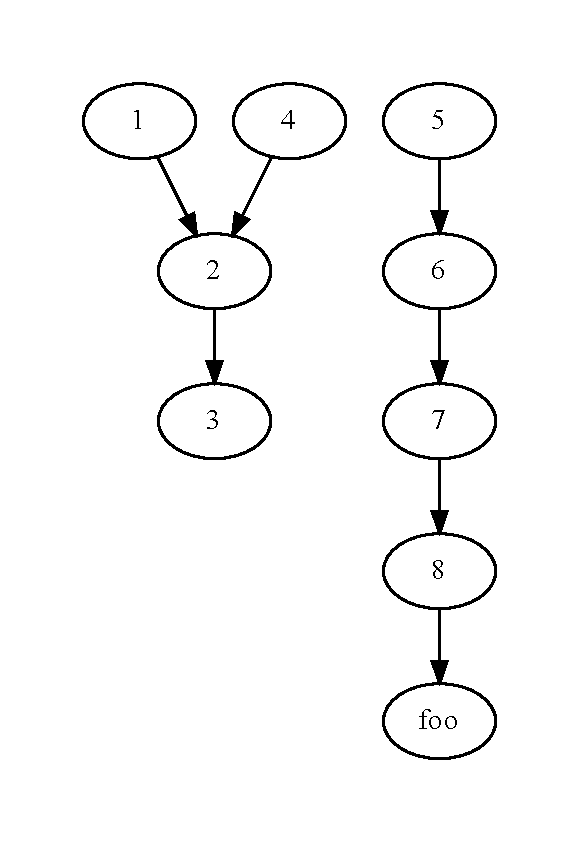
\includegraphics[scale=0.5]{cfg.pdf}
        \end{center}
        \caption{Initial CFG}
\label{fig:cfg0}
\end{figure}
Hypothetically circumscribing over the $\pred{successor}{\cdot, \cdot}$ predicate representing known transitions gives us a ``complete'' control flow graph to pass to a value analysis.
This circumscription assumed that $\forall{X}. \neg \pred{successor}{3, \var{X}}$.
However, the value analysis will quickly determine that \texttt{eax} may hold 4, and so finds $\pred{successor}{3, 4}$.
At this point, the informal version of this analysis reasons that since $\neg \pred{successor}{3, 4}$ contradicts itself, the next step is to assume $\pred{successor}{3, 4}$.\footnote{\
        It is actually possible to avoid reasoning from contradiction here: since VSA\cite{vsa} will only widen its value upper bound in response to new edges, and new edges are being discovered via these upper bounds, at a minimum those edges found in the current graph will be found in the true graph.
        However, VSA is still nonmonotonic, since the upper bounds it produces are invalidated (since they could become wider).
        Without modeling a property only present in composition, contradiction-based reasoning is unavoidable.
}

%   * Why is this call-CC?
One way to express such an ability would be to tie it to the law of excluded middle: $A \vee \neg A$.
However, an equivalent property $((A \imp \bot) \imp A) \imp A$ better captures the action of the evaluation procedure conceptually.
First, the evaluator guesses that $A$ cannot happen during the circumscription, i.e. $(A \imp \bot)$.
From that, it derives $A$.
As a result, outside the circumscribed world, we want $A$ to be visible as a fact.

% Bidirectional Proof Search
\section{Bidirectional Proof Search}
\label{sec:bidisearch}
In the background, I reviewed forwards (\S~\ref{sec:fchain}) and backwards (\S~\ref{sec:bchain}) chaining analyses.
Which to use is generally selected situationally, but I argue that for our use case, both are needed.
% * Forwards chaining = datalog
\subsection{Forwards Chaining}
Forwards chaining corresponds to the simpler ``do this when possible'' style of organization that program analysis authors are likely more familiar with.
%   * Want this to represent things which
%     * Almost always need to be done
It is good for representing things that will nearly always need to be done,
%     * Can be done efficiently
can be done efficiently,
%     * Have a reasonably bounded extent
and whose extent is reasonably bounded.
If the analysis does not usually need to be done, it will fire when it does not need to.
If it cannot be done efficiently, it will burn resources that may be needed elsewhere.
If its extent is not reasonably bounded, the analysis will pollute the database with a large morass of facts.

%   * Examples
There are several good examples of analyses which fit the forward chaining mold well.
%     * Parse
Parsing the binary container format will need to be done before nearly every other kind of analysis, is quite fast, and will produce facts bounded linearly in the size of the input binary.
%     * Lifting
Lifting of an address identified as executable will nearly always be needed to make any further queries about it, is a constant time operation per address, and produces a bounded data value.

%   * Good for preprocessing/directed auto-analysis
Overall, forwards chaining gives a good representation of what is normally viewed as preprocessing or auto-analysis.

% * Backwards chaining = prolog
\subsection{Backwards Chaining}
Backwards chaining corresponds to the ``do this when needed'' strategy of execution analogous to what occurs in user facing analysis tools or program property checker.
%   * Want this to represent things which
Backwards chaining is more appropriate for representing analyses which
%     * Rarely need to be done
are rarely needed,
%     * Are potentially expensive
are potentially expensive to run,
%     * Have an enormous or infinite extent
or have a large (or infinite) extent.

%   * Examples
While I expect most basic functionality to work well as forward-chaining analyses, some standard techniques simply do not fit well with it.
%     * Fuzz
Fuzzing is possibly one of the clearest cases.
A fuzzing run generates a vast amount of data, and can potentially generate an arbitrary amount by triggering with new random values.
These runs are also generally expensive.
%     * Solve this function for stack overflow with symex + smt
Another example of an analysis that fits better with backwards chaining is property checking via symbolic execution and SMT solving.
While the extent is small, it is potentially slow and has a wide variety of potential entry points/properties, very few of which are actually interesting.
% * Execution strategy
\subsection{Execution Strategy}
While my execution strategy is largely informed by my implementation strategy, it still reflects similar semantics to what is seen in the inspiration languages.
%   * Queries / rule firing acts as a transaction, multiple may be in flight
First, rule firings are treated as transactions, with conflicts being negotiated by the database.
This allows for a good deal of parallelism because with the exception of circumscription, no conflicting writes should occur to the database.
The one apparent downside of this is that analyses may potentially need to be rolled back (especially if they take longer to finish) if the database had a conflicting update via a circumscription.
However, had the same operations been performed in order, the run would still have been invalidated eventually.
In parallel, using transactions, Holmes will
\begin{itemize}
%   * Try to fire any legal forwards chaing rules until quiescence
\item Run any forwards chaining rules which have new body matches.
%   * If a query is received
\item If a query is recieved,
        \begin{enumerate}
%     * Output known matches
                \item Output known matches
                \item Add a goal root to the database for the given goal if not already present.
                \item Upon a request for more, give any new results present to the client
                \item Upon termination, decrement the goal root refcount or remove it if this is the only request.
        \end{enumerate}
\item Perform a tabling backwards search\footnote{\
                Strategy is to be decided, but may be anything from rule order to previous execution time, to a learning system.
        } for any root goals whose search has not been completed.
\end{itemize}

\section{Semantics}
To give a slightly more formal view of what I expect this system to do, I provide a derivability relation.
These rules are rough, but I hope they will help make my intentions more clear.

In these rules, the $\Gamma$ context is a bag context that is allowed weakening only when $\Delta$ is empty.
$\Gamma$ represents monotonically true facts and rules, a context of immutable truth.
$\Delta$ is an ordered context.
$\Delta$ is used to contain assumptions made thus far, with the rightmost assumption being the most recent.
$P^\tau$ and similar expressions are used to represent a predicate which has $\tau$ used as a free variable.
$E[x/y]$ is used to represent the substitution of $y$ for $x$ in the expression $E$.
I use $\vec{x}$ throughout to act as a shorthand for $x_1 \ldots x_n$.
\newcommand{\ds}{\vdash}
\begin{gather*}
  \infer[id]{\Gamma, a : P; \Delta \ds a : P}{}\\
  \infer[xchg]{\Gamma_0, x, \Gamma_1, y, \Gamma_2; \Delta \ds z}{\Gamma_0, y, \Gamma_1, x, \Gamma_2; \Delta \ds z}\\
  \infer[weaken]{\Gamma, x; \cdot \ds y}{\Gamma; \cdot \ds y}\\
  \infer[rule]{\Gamma, r : \forall \tau_0 \ldots \tau_n. ((P_1^{\vec{\tau}} \ldots P_m^{\vec{\tau}}) \rightarrow Q^{\vec{\tau}}); \Delta \ds r(\vec{\sigma}, \vec{p}) : Q^{\vec{\tau}}[\vec{\tau}/\vec{\sigma}]}{\Gamma; \Delta \ds p_1 : P_1^{\vec{\tau}}[\vec{\tau}/\vec{\sigma}] & \cdots & \Gamma; \Delta \ds p_m : P_m^{\vec{\tau}}[\vec{\tau}/\vec{\sigma}]}\\
  \infer[monagg]{\Gamma; \Delta \ds \{\vec{a}\} : P^\tau[\tau/(\leq \rho)]}{\Gamma; \Delta \ds a_1 : P^\tau[\tau/\sigma_1] & \cdots & \Gamma; \Delta \ds a_n : P^\tau[\tau/\sigma_n] & \bigvee \vec{\sigma} \leq \rho}\\
  \infer[hypcirc]{\Gamma; \Delta\vdash [\vec{a}] : (|\tau. P^\tau| = \vec{\sigma}) \Rightarrow P^\tau[\tau/\vee = \rho]}{\Gamma; \Delta \ds a_1 : P^\tau[\tau/\sigma_1] & \cdots & \Gamma; \Delta \ds a_n : P^\tau[\tau/\sigma_n] & \bigvee \vec{\sigma} = \rho}\\
  \infer[assume]{\Gamma; \Delta,  |\tau. P^\tau| = \vec{\sigma} \ds e : Q}{\Gamma; \Delta \ds e: (|\tau. P^\tau| = \vec{\sigma}) \Rightarrow Q & \forall a : P^\tau[\tau/\rho] \in \Gamma. \rho \in \vec{\sigma}}\\
  \infer[unassume]{\Gamma; \Delta \ds e : (|\tau. P^\tau| = \vec{\sigma}) \Rightarrow Q}{\Gamma; \Delta, (\vec{\sigma}, \tau, P^\tau) \ds e : Q}\\
  \infer[callcc]{\Gamma; \Delta, |\tau. P^\tau| = \vec{\sigma'} \ds callcc(e, e') : P^\tau[\tau/\vee = \rho']}{
    \begin{array}{ccc}
      \vec{\sigma'} = \vec{\sigma} + \gamma & \rho' = \rho \vee \gamma & \gamma \not \in \vec{\sigma} \\
      \Gamma; \Delta, |\tau. P^\tau| = \vec{\sigma} \ds e : P^\tau[\tau/\gamma] & & \Gamma; \Delta, |\tau.P^\tau|=\vec{\sigma} \ds e' : P^\tau[\tau/\vee = \rho]
  \end{array}}
\end{gather*}
The first three rules (id, xchg, weaken) establish the basic framework in which we are working (as per the context explanations above).

The ``rule'' rule expresses the basic way in which rules can be applied to facts.
This rule is similar to parametrically polymorphic function application.
The primary difference is that $Q$'s expression may contain an invocation of an external function, and so until the selection of the type paramter vector $\vec{\tau}$, you can't actually know what type the proof term has.

The ``monagg'' rule describes monotonic aggregation.
I use the notation $\leq \rho$ to represent a value for which we know that the meet of all values is at least less than $\rho$.
In actual use, you'd likely see e.g., $P(1, \leq \{2, 3\})$ or something similar.
The rule itself essentially says that if you have a proof for $P^\tau$ with each of a nubmer of different options, and their meet is less than some bound, then their set comprises a proof of $P^\tau$ with $\tau$ monotonically aggregated to $\rho$.

The ``hypcirc'' rule describes the procedure for hypothetical circumscription.
The construct $|\tau.P^\tau| = \vec{\sigma}$ is meant to represent that the total extent of assignments to $\tau$ for which $P^\tau$ may be derived is $\vec{\sigma}$.
This can be thought of (roughly, this is informal) as $\not \exists \gamma. (\gamma \not \in \vec{\sigma}) \wedge \Gamma; \Delta \vdash e : P^\tau[\tau/\gamma])$
What hypcirc allows is the use of the meet of a set of possible assignments to $\tau$ as an approximation of the true meet of all assignments, with the assumption added to the type.

The rules ``assume'' and ``unassume'' help guide search.
The ``assume'' rule is for limited movement of an assumption from the type of a proof term into the context.
The ``unassume'' rule inverts assume, but is unlimited, since we are not limited in what assumptions may occur on the right of the turnstile.
``assume'' in particular is very much not in its final form.
Currently, it only allows movement from the left hand side of a $\Rightarrow$ to the $\Delta$ context if there is not an identity-based proof of its assumption being wrong.
In a more complete version of this rule, the premises would contain a stronger notion of the concept of having failed, potentially temporarily, to produce contradictory proofs despite trying.
In this way, hypothetical circumscriptions which can be absorbed into the assumption context will be similar to stratified negation.
The primary difference between a limited assume and stratified negation will be that it is more permissive in what having tried hard enough to derive the fact is before it is allowed to assume it is false.

``callcc'' implements the assumption expansion in case of contradiction discussed previously (\S \ref{sec:callcc}).
If we can derive a contradiction to the most recent assumption, the $callcc$ constructor allows us to update the meet based on the knowledge of the flawed assumption.
It takes in a proof of a contradiction of the assumption, a predicate derived from the meet of that assumption, and updates it to contain the new information.

While these rules are rough, I hope they serve to give an idea of the intended derivability relationship.
\section{Implementation Strategy}
\label{sec:impl}
As I've begun the implementation of this system, I have already made several design decisions.

% * Lang = rust
%   * Safe
%   * Efficiently handles large data
%   * Threading story
For implementation of the logic engine itself, I have decided to use Rust\cite{rust}.
Rust is a safe, multithreaded language which provides C/C++ style direct control of allocation, copies, and other such processes.
This means that while I will not suffer as much overhead as more traditional safe languages, I will not be plagued by the issues I had with an initial C++ prototype.\footnote{\
        Combining C++ closures for asynchronous callbacks with multithreading brings up a number of surprising edge cases, none of which are checked for by the compiler.
        This was consuming too much development time, and I forecasted it would only get worse.
}

% * Database engine = postgres
To hold the data, I've selected Postgres.
%   * Transactions (multiple rules in flight)
%   * Joins (avoid writing a custom query compiler for match terms, just compile to joins)
Like most modern SQL systems, Postgres supports transactions and joins.
Transactions are important to allowing multiple rules in flight, as they provide clean synchronization.
Joins allow me to compile the match clauses of rules into SQL queries, substantially speeding up search in larger databases.\footnote{\
        An earlier naive in-memory prototype was actually much slower despite the faster access speed.
I made the decision to use a database layer when I realized the indexing code I was about to begin writing was roughly equivalent to the code in a standard SQL database.
}
%   * Efficient jsonb support for custom user data structures
Finally, Postgres is unique in providing efficiciently indexable, binary stored \texttt{JSON} objects through its \texttt{jsonb} extension.
While this will not be required initially, it will make allowing user defined datatypes, especially ASTs and similar structures, much easier later.

% * RPC system = Cap'n'proto
To bind analyses to the logic engine to allow their functions to be called, I either need to link them in, load shared libraries, or use an RPC system.
I ruled out linking in to allow for interpreted languages and avoid recompilation.
Plugins (shared library building) were ruled out because they are tricky for potential developers to build, and would again rule out interpreted languages.
As a result, \sysname\ requires an RPC system.
To fill this gap, I selected Cap'n Proto\cite{capnproto}, a system from a creator of Google's Protobuf\cite{protobuf}.
The primary reasons for selecting Cap'n'proto were multilanguage support, capability support, efficiency, and embeddability of dynamic structures.
Supporting many languages will ease the writing of analyses for \sysname.
Capability support both allows analyses to easily follow a ``registration'' pattern (sending an object to the server constructed with the relevant callbacks), and allows for lazy reading of large values such as traces or process image dumps.
Efficiency of the encoding is important to allow for the transfer of larger objects involved in binary analysis, such as traces\footnote{\
Traces are regularly many gigabytes in size.
}
The ability to embed dynamic structured binary data through reflection will make it easier to support analysis-defined types later on in the effort.

% * See impl in progress at my github
You can view the implementation in progress on GitHub.\footnote{\url{http://github.com/maurer/holmes}}

\chapter{Conclusion}

\backmatter
\renewcommand{\bibsection}{\chapter{\bibname}}
\bibliographystyle{alphaurl}
\bibliography{proposal,aux}

\end{document}
